\documentclass{article}
% \title{A_AgarwalKapoorMudgal}
% if you need to pass options to natbib, use, e.g.:
% \PassOptionsToPackage{numbers, compress}{natbib}
% before loading nips_2016
%
% to avoid loading the natbib package, add option nonatbib:
% \usepackage[nonatbib]{nips_2016}

\usepackage[final]{nips_2016}
\usepackage{graphicx}
\usepackage[font=small,labelfont=bf]{caption} % Required for specifying captions to tables and figures
% to compile a camera-ready version, add the [final] option, e.g.:
% \usepackage[final]{nips_2016}

\usepackage[utf8]{inputenc} % allow utf-8 input
\usepackage[T1]{fontenc}    % use 8-bit T1 fonts
\usepackage{hyperref}       % hyperlinks
\usepackage{url}            % simple URL typesetting
\usepackage{booktabs}       % professional-quality tables
\usepackage{amsfonts}       % blackboard math symbols
\usepackage{nicefrac}       % compact symbols for 1/2, etc.
\usepackage{microtype}      % microtypography
\usepackage{amsmath}

\title{Learning to Project Multiple Modalities to a Common Subspace}

% The \author macro works with any number of authors. There are two
% commands used to separate the names and addresses of multiple
% authors: \And and \AND.
%
% Using \And between authors leaves it to LaTeX to determine where to
% break the lines. Using \AND forces a line break at that point. So,
% if LaTeX puts 3 of 4 authors names on the first line, and the last
% on the second line, try using \AND instead of \And before the third
% author name.

\author{
Aayush Mudgal \\
%   Aayush Mudgal\thanks{\href{http://aayushmudgal.github.io}{Homepage}} \\
  Department of Computer Science\\
  Columbia University\\
  New York, NY 10027 \\
  \texttt{am4590@columbia.edu} \\
  %% examples of more authors
  \And
  Mridul Kapoor \\
  Department of Computer Science\\
  Columbia University\\
  New York, NY 10027 \\
  \texttt{mk3908@columbia.edu} \\
  \AND
  Tushar Agarwal\\
  Department of Computer Science\\
  Columbia University\\
  New York, NY 10027 \\
  \texttt{ta2482@columbia.edu} \\
  %% \And
  %% Coauthor \\
  %% Affiliation \\
  %% Address \\
  %% \texttt{email} \\
  %% \And
  %% Coauthor \\
  %% Affiliation \\
  %% Address \\
  %% \texttt{email} \\
}

\begin{document}
% \nipsfinalcopy is no longer used

\maketitle

\begin{abstract}
In recent years, cross modal retrieval has drawn much attention due to the easy and wide availability of multi-modal data. Here we basically look at audio and the corresponding video features, and map them to a common feature space which is more informative than the original feature space. We propose an iterative algorithm that learns this mapping by alternatively learning a better projection and a more discriminative classifier. A live demo of our cross-modal retrieval system is available \href{http://audioset.herokuapp.com/}{here}
\end{abstract}

\section{Introduction}

Video data is something that is very easily captured, it would be quite beneficial if we could analyze it better. Typically the video data resides in a very high dimension as compared to the audio. It is also expected that any algorithm that utilizes the information from both these modalities, should at least work similar or better than using only one of the modalities. Thus it is very important to learn a good common subspace where we can project these modalities, and use them for improved performance. Currently, a lot of deployed video search and retrieval is based upon user-provided text attributes such as title and description. Better representation learning would in effect help in better video-search and retrieval. Such common subspaces would also help in improved tagging and classification of videos, as it would incorporate information from both the video and audio features. We propose an alternating iterative algorithm that learns a common representation for the audio and video modalities. The proposed algorithm iteratively minimizes the mean squared classification error in one step, and the resulting KL Divergence of the learned common space with respect to  one of the modalities as the next step.

\section{Datasets}

\subsection{AudioSet}
AudioSet \cite{audioset} is a sound vocabulary and dataset, just released by Google in February 2017. It consists of an expanding ontology of 632 audio event classes and a collection of over 2 million human labeled 10-second sound clips drawn from YouTube videos. It specifies the ontologies as a hierarchical graph of event categories, covering a wide range of human and animal sounds, musical instruments and genres and also common everyday sounds. For the purpose of our experiments we filtered audio data corresponding to the 128 major ontological classes. 

128 dimensional audio features for every second of video, generated through a VGG inspired neural network, were provided as a part of the dataset. Since the dataset did not contain the video features, we manually downloaded the corresponding videos from YouTube, and generated the corresponding frame-level features using the state-of-the-art publicly available VGG16 Network \cite{vgg16} trained on Imagenet \cite{imagenet}. This generated 4096 dimensional video features for every 0.5 seconds of the video. 

\subsection{YouTube 8M}
Google's YouTube 8M  \cite{youtube8m}  is the benchmark dataset for video understanding. It consists of over 3.2 billion audio/video features covering 4716 classes from 0.45 million hours of YouTube videos. It comes with pre-extracted audio (128 dimensional) and visual (1024 dimensional) features from every second of YouTube videos (3.2B feature vectors in total). 


\section{Related Work}
\begin{center} 
\begin{figure}[h]
\label{fig:overview1}
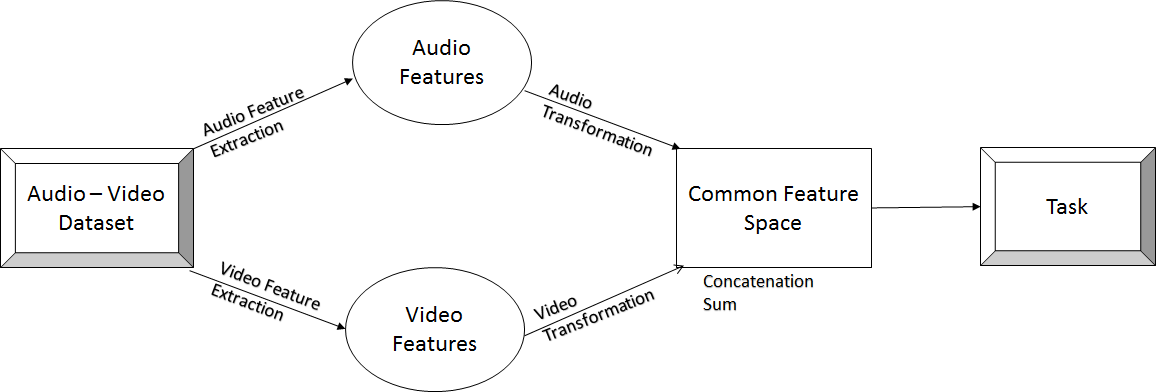
\includegraphics[width=1\textwidth]{figures/overview.png}
\caption{Overview of General Feature Fusion Algorithms}
\end{figure}
\end{center}

\cite{review} provides a good overall review of the recent and relevant work in the space of cross modal retrieval and representation learning. The representative methods for cross-modal retrieval can be divided into two types: 1) Real Valued Representation Learning and 2) Binary Representation Learning. The Real Valued Representation Learning aims to learn a real valued common representation for the different modalities. Binary representation Learning methods are proposed to speed up cross-modal retrieval, by mapping different modalities into a common Hamming space. Most existing methods \hyperref[fig:overview1]{(see figure)} try to learn a transformation matrix from the respective cross modal spaces into a new projected space, where they share the same dimensions. In the projected common feature space, they generally fuse by either concatenation or summation over the projected features.

The two most widely used strategies for multi-modal fusion are Canonical Correlation Analysis (CCA) \cite{cca} and Discriminant Correlation Analysis (DCA) \cite{dca}. We present a brief introduction of each. We also discuss our proposed iterative algorithm that alternatively minimizes the classification error, and KL Divergence between the projected features and one of the features. Finally, we present the results of classification achieved using these projected features through different algorithms. We observe that our proposed model, performs significantly better than the existing techniques.

\subsection{Canonical correlation analysis}
The Canonical correlation Analysis (CCA) \cite{dca_1}, a statistical method has been widely used to explore relationships between two multivariate sets of variables measured on the same individual. Alternatively it can be defined as the problem of finding two sets of basis vectors, one for each multivariate \textbf{X} and \textbf{Y} such that the correlations between their projections onto the basis vectors are mutually maximized.


Let X$\epsilon$$R^{s\times n}$ and Y$\epsilon$$R^{t\times n}$, be two matrices, each containing n features but belonging to different modalities. Let $S_{xx} \epsilon R^{s\times s}$ and $S_{yy} \epsilon R^{t\times t}$ denote the the within sets covariance matrices of X and Y while $S_{xy} \epsilon R^{s\times t}$ denotes the between sets covariance matrix. Note that, $S_{xy}$ = $S_{yx}^T$. CCA finds the linear combinations $\hat{X} = W_x^T X$ and $\hat{Y} = W_y^T Y$ which maximizes the pairwise correlation between feature sets X and Y. The transformation matrices $W_x$ and $W_y$ are found by solving the following sets of equations:

% \[ \begin{cases} 
\begin{gather*}
S_{xx}^{-1}S_{xy}S_{yy}^{-1}S_{yx}\hat{W}_x = R^2\hat{W}_x \\ 	S_{yy}^{-1}S_{yx}S_{xx}^{-1}S_{xy}\hat{W}_y = R^2\hat{W}_y
\end{gather*}
% \]

Where $\hat{W}_x$ and $\hat{W}_y$ are eigenvectors and $R^2$ consists of squares of the canonical correlations (diagonal matrix of eigenvalues). After obtaining the transformed feature sets $\hat{X}$ and $\hat{Y}$, feature fusion is obtained either by concatenation or summation of the transformed feature vectors. From the t-sne visualizations \ref{fig:cca}, we can see that features in the fused feature space significantly separates out the different labels, as compared to individual features alone. 
\begin{center}
\begin{tabular}{cc}
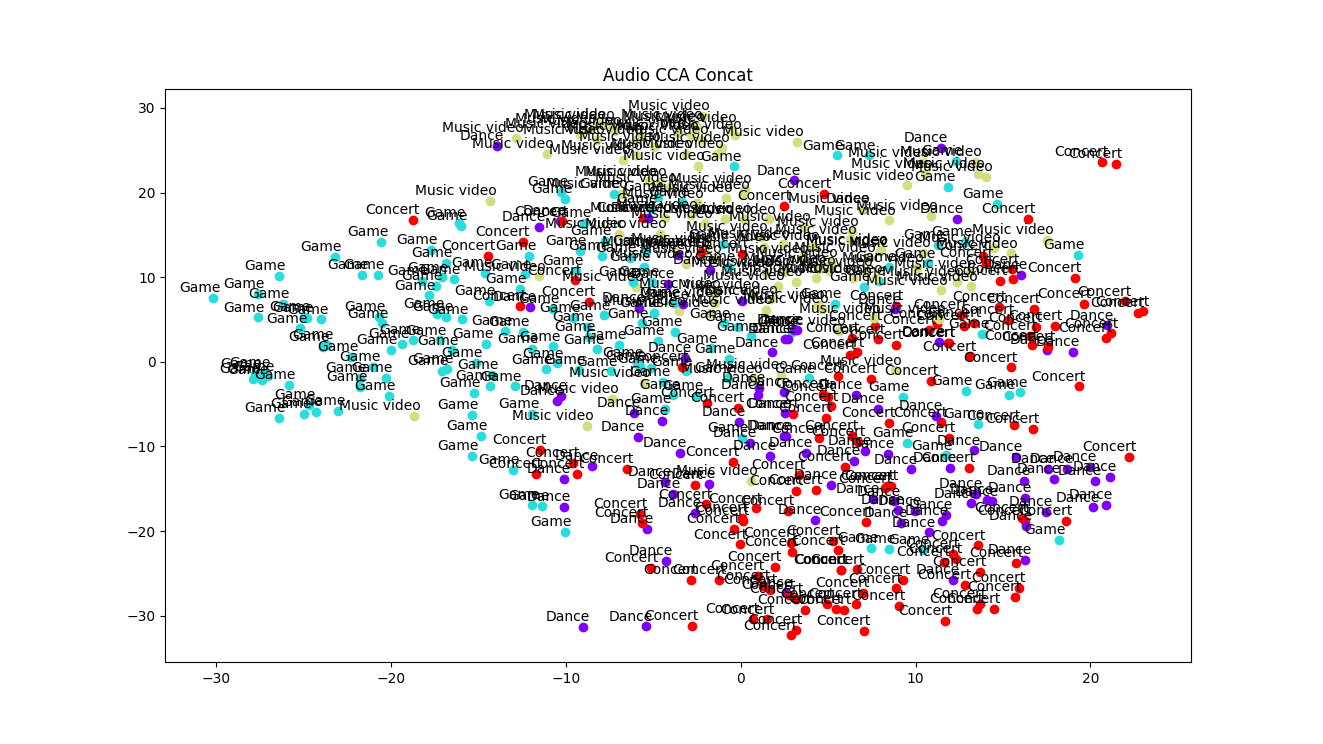
\includegraphics[width=0.49\linewidth]{figures/c_c_a.png} &
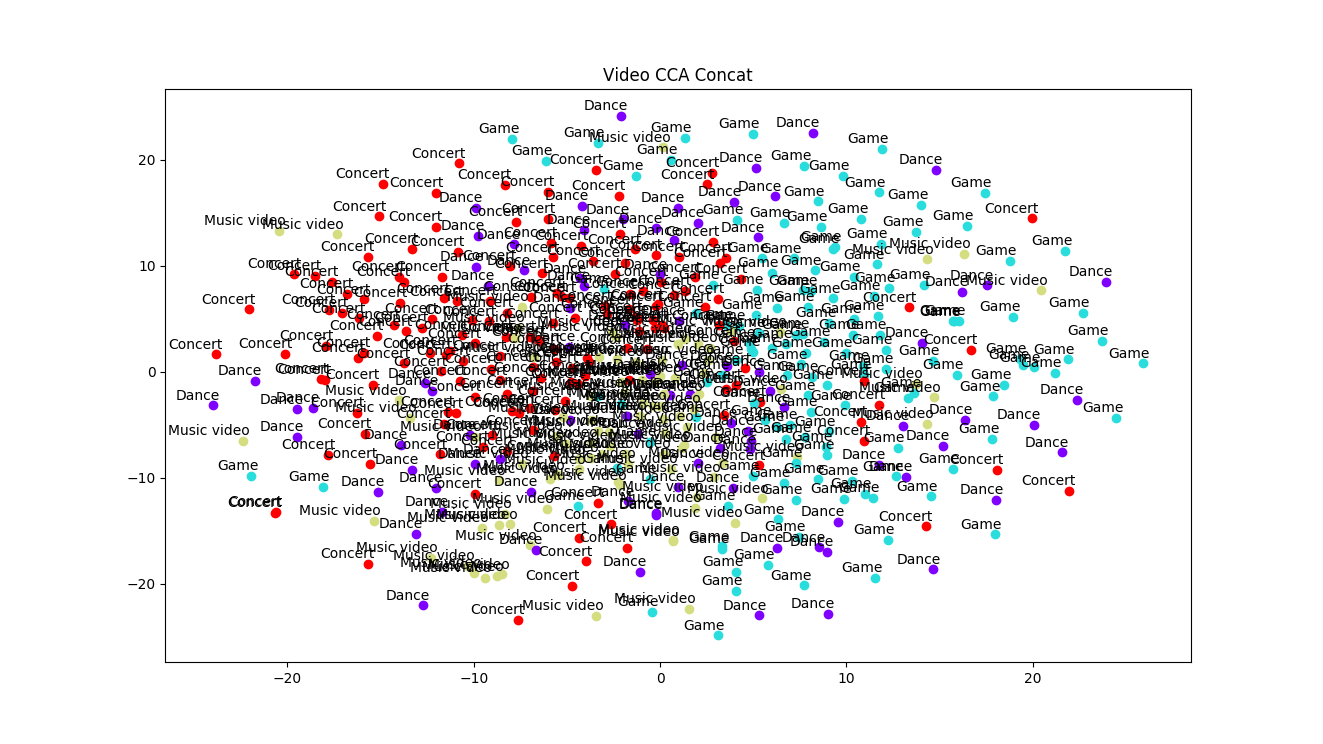
\includegraphics[width=0.49\linewidth]{figures/c_c_v.png} \\
 a) & b)\\
 \end{tabular}
 \begin{tabular}{c}
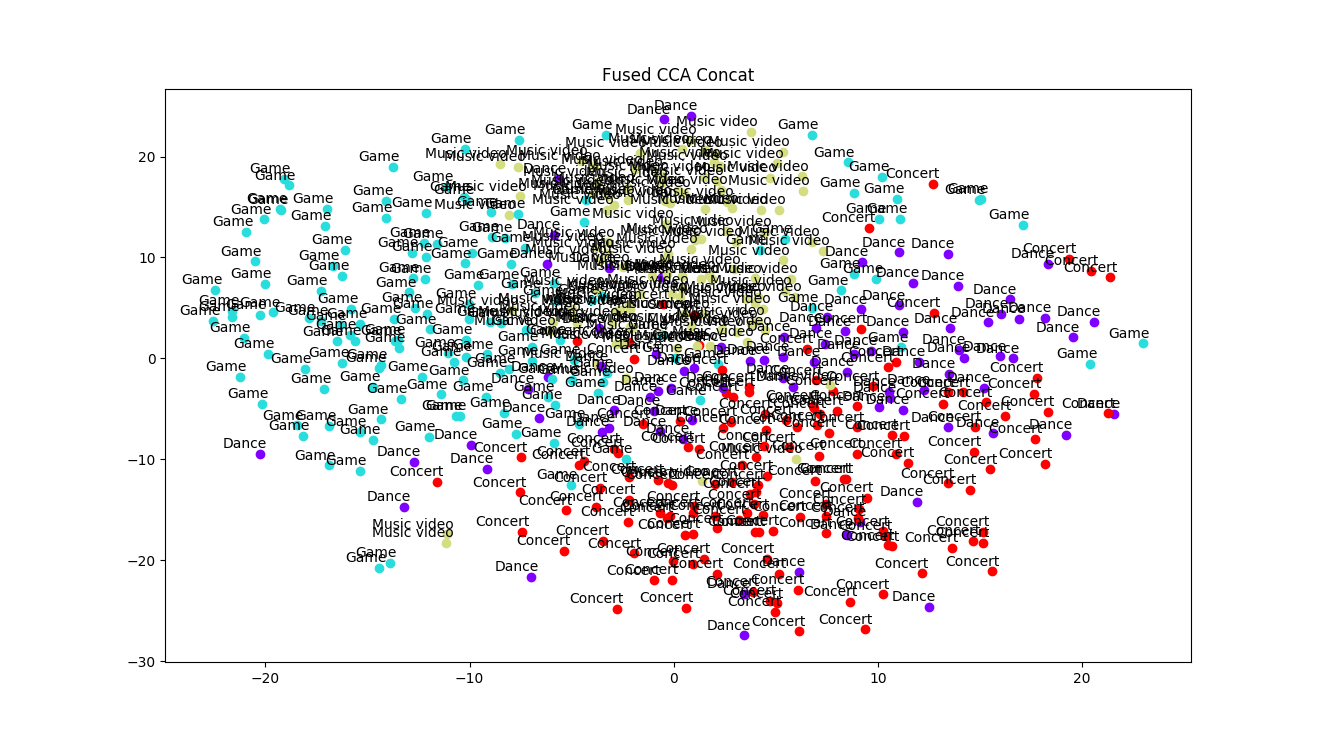
\includegraphics[width=0.49\linewidth]{figures/c_c_f.png} \\
 c)\\
 \end{tabular}
 \label{fig:cca}
\captionof{figure}{t-SNE visualizations of 1000 data points corresponding to Dance (Red), Concert (Yellow), Game (Purple) and Music (Blue). (a): Visualization of Audio Features Only. (b): Visualization of Video Features Only, (c): Visualization of Fused Features after CCA}
 \end{center}
% \begin{figure}[h]
% \centering
% 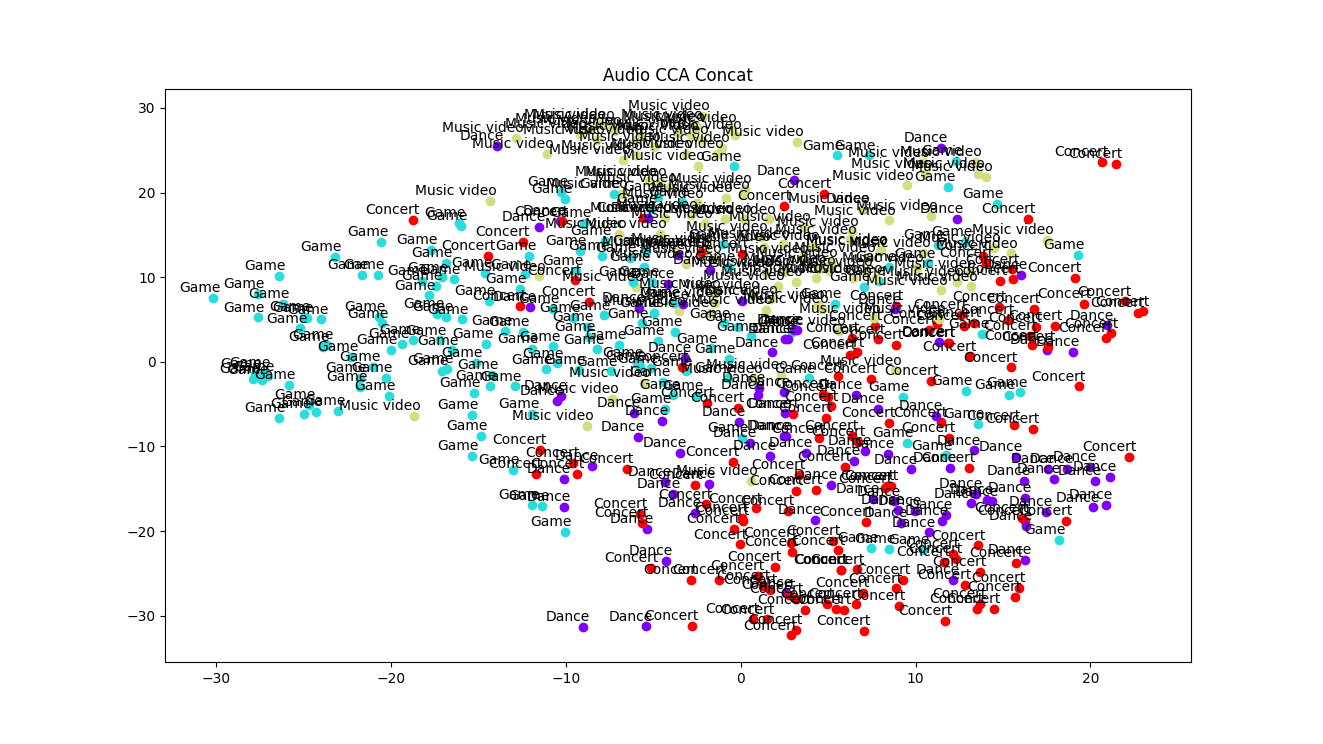
\includegraphics[width=.5\textwidth]{figures/c_c_a.png}\hfill
% 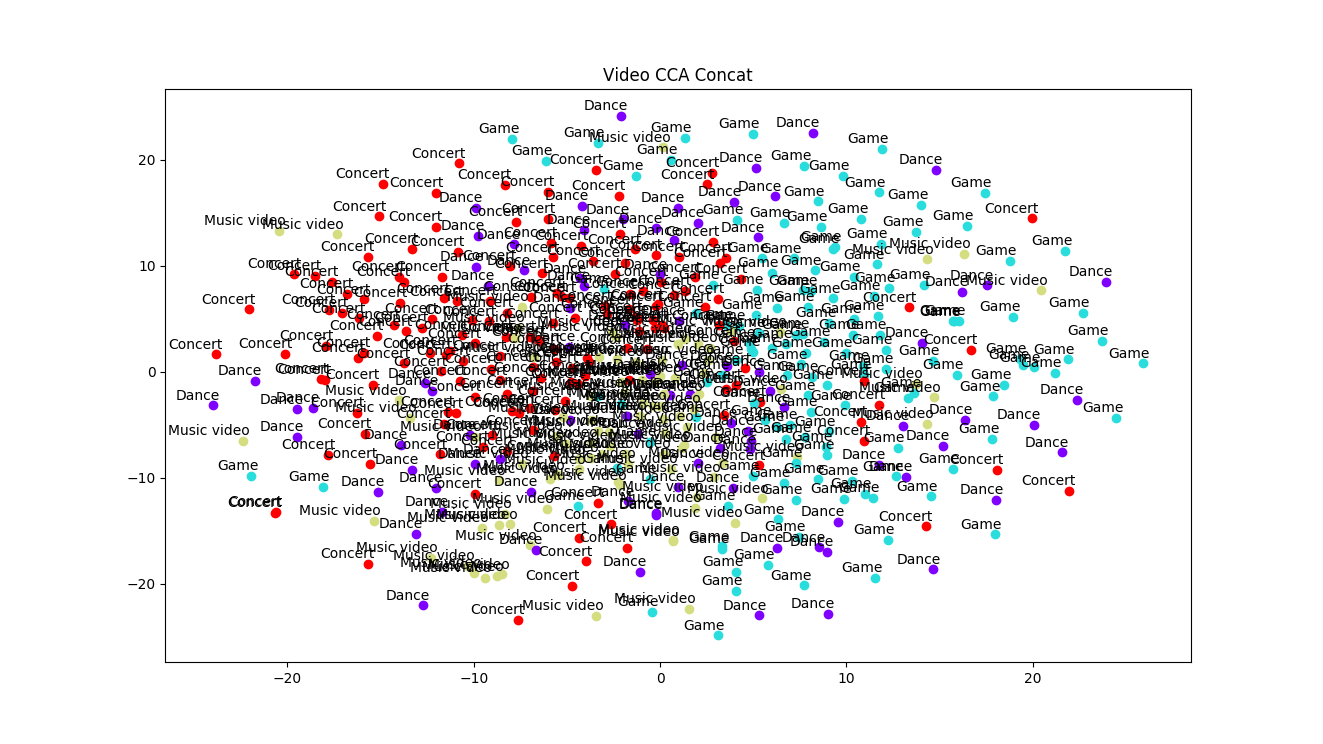
\includegraphics[width=.5\textwidth]{figures/c_c_v.png}\hfill
% 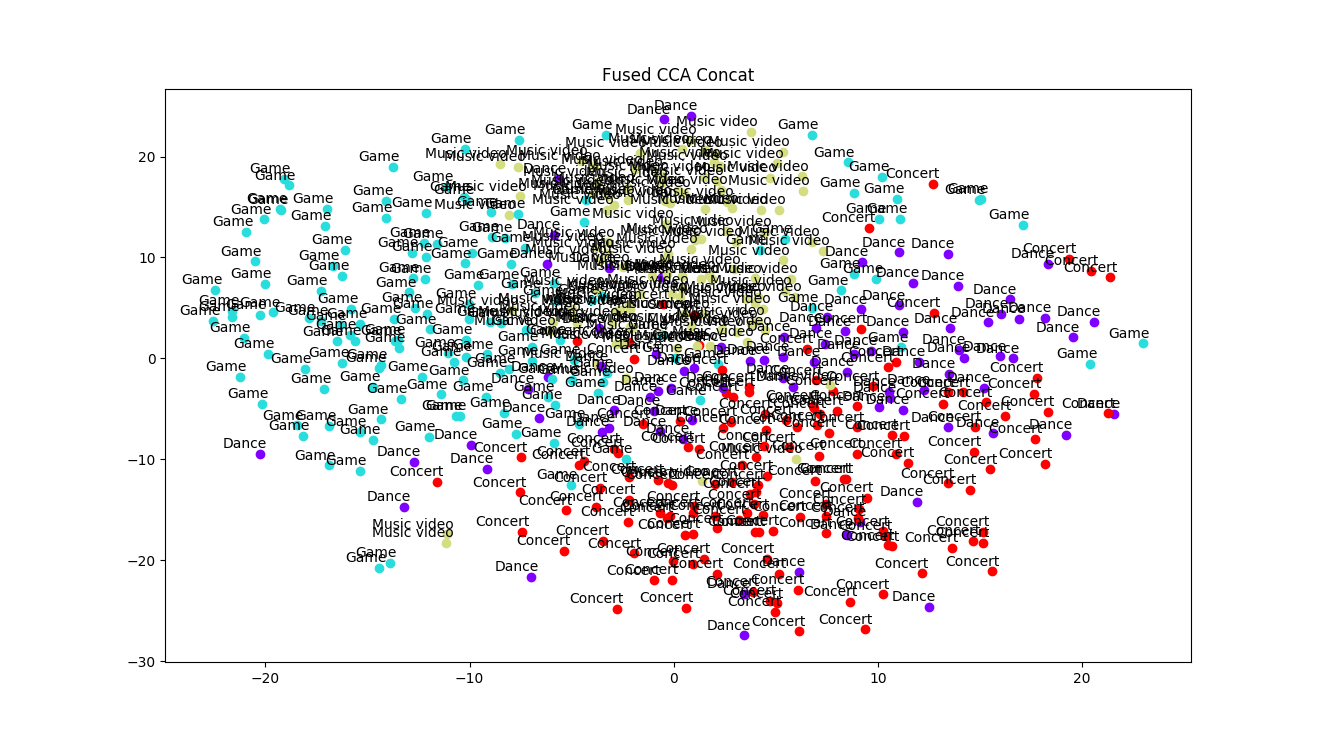
\includegraphics[width=.5\textwidth]{figures/c_c_f.png}
% \caption{}
% \label{fig:cca}
% \end{figure}

We used a 5 fold cross validation and kernalized SVM and extreme gradient boosting as classification algorithms, to test the performance of the transformed features. The results are then compared to initial features described in the \ref{results-table}. \footnote{The code and metrics for the trained models, as well as that for featurization can be found on the \href{https://github.com/mridul/project-adv-ml}{our github repository}}

\subsection{Discriminant Correlation Analysis}
Unlike CCA, DCA \cite{dca} is a supervised strategy for multi-modal feature fusion. It aims to maximize the pair-wise correlations across the two feature sets X and Y, while it also eliminates the between-class correlations at the same time. It thus restricts the correlations to be within classes.

Traditionally DCA has been used for the fusion of biometrics data. It has found varied applications in pattern recognition problems that involve fusing features extracted from multiple modalities or multiple features from single modality. As an example DCA is commonly used to identify a person using features obtained from multi-modal sources such as fingerprint and iris scans. It has very low computational complexity and can be easily used for real-time applications. 

Let us consider a data matrix in which the samples are collected from c different classes. This means that the n columns of the data matrix are divided into c different groups where $n_i$ columns belong to the $i^{th}$ class. Let $x_{ij}\epsilon X$ denote the feature vector which corresponds to the $j^{th}$ sample in the $i^{th}$ class. Therefore:
\begin{gather*}
  \tilde{x}_i = \frac{1}{n_i}\Sigma_{j=1}^{n_i}x_{ij} \qquad\text{$\Rightarrow$}\qquad \tilde{x} = \frac{1}{n}\Sigma_{i=1}^c\Sigma_{j=1}^{n_i}x_{ij} = \frac{1}{n}\Sigma_{i=1}^{c}n_{i}\tilde{x}_i
\end{gather*}
\iffalse
$\tilde{x}_i$ = $\frac{1}{n_i}\Sigma_{j=1}^{n_i}x_{ij}$\\
$\tilde{x}$ = $\frac{1}{n}\Sigma_{i=1}^c\Sigma_{j=1}^{n_i}x_{ij}$ = $\frac{1}{n}\Sigma_{i=1}^{c}n_{i}\tilde{x}_i$\fi
where $\tilde{x}_i$ and $\tilde{x}$ represent the means of the $x_{ij}$ vectors in the $i^{th}$ class and in the complete feature set.

The between class scatter matrix is defined as:\\
\begin{gather*}
S_{bx_{(p\times p)}} = \Sigma_{i=1}^c n_i(\tilde{x}_i - \tilde{x})(\tilde{x}_i - \tilde{x})^T = \phi_{bx}\phi_{bx}^T\\
where ~~ \phi_{bx_{(p \times c)}} = [~ \sqrt[]{n_1} 
 (\tilde {x}_1 - \tilde x),\sqrt[]{n_2} (\tilde x_2 - \tilde x ),.....,\sqrt[]{n_c} ( \tilde x_c - \tilde x ) ]
\end{gather*}
\iffalse

If the classes are well-separated then $\phi_{bx}^T\phi_{bx}$ will be a diagonal matrix. Since $\phi_{bx}^T\phi_{bx}$ is symmetric positive semidefinite,
the transformations that diagonalize it are as follows:
\begin{gather*}
P^T\phi_{bx}^T\phi_{bx}P = \hat{\wedge}
\end{gather*}\\
where P is the matrix of orthogonal eigenvectors and and $\hat{\wedge}$ represents the
diagonal matrix of eigenvalues sorted in decreasing order.

Next, $Q_{(c\times r)}$ be a matrix which contains the first r eigenvectors corresponding to the r largest nonzero eigenvalues from the matrix P. We get:\\
$Q^T\phi_{bx}^T\phi_{bx}Q$ = $\wedge_{(r \times r)}$

The r most significant eigenvectors of $S_{bx}$ can be obtained by mapping: Q$\rightarrow \phi_{bx}Q $ as:\\
$(\phi_{bx}Q)^T S_{bx} (\phi_{bx}Q)$ = $\wedge_{(r \times r)}$
\fi
The transformation $W_{bx = }(\phi_{bx}Q)\wedge^{\frac{-1}{2}}$ unitizes $S_{bx}$ 
and reduces the dimensionality of the data matrix X from p to r as shown below:\\
\begin{equation*}
  W_{bx}^T S_{bx}W_{bx} = I \qquad\text{$\Rightarrow$}\qquad X'_{(r \times n)} = W_{bx_{(r \times p)}}^TX_{(p \times n)}
\end{equation*}
\iffalse
$W_{bx}^T S_{bx}W_{bx} = I$\\$X'_{(r \times n)} = W_{bx_{(r \times p)}}^TX_{(p \times n)} $\\

Here, $X'$ is the projection of X in a space where the between classes scatter
matrix is I and the classes of X are separated. 

$W_{by}^T S_{by}W_{by} = I$\\$Y'_{(r \times n)} = W_{by_{(r \times q)}}^TY_{(q \times n)} $

Now, although $S'_{bx}$ = $S'_{by}$ = I, the matrices $\phi_{bx}^{'T} \phi'_{bx}$ and $\phi_{by}^{'T} \phi'_{by}$ are matrices which are strictly diagonal. This results in  the centroids of the classes to have minimal correlation with each other and thus are separated. Now since the between classes scatter matrices have been unitized, we need
to ensure that the features in one set have nonzero correlation only with
their corresponding features in the other set. To achieve this we
diagonalize the between set covariance matrix $S'_{xy}= X'Y^{'T}$. We compute SVD for this as:\\
\fi
Similarly for feature set Y we get:
\begin{equation*}
  W_{by}^T S_{by}W_{by} = I \qquad\text{$\Rightarrow$}\qquad Y'_{(r \times n)} = W_{by_{(r \times q)}}^TY_{(q \times n)} 
\end{equation*}
To ensure that the features in one set have nonzero correlation only with the corresponding features in this set we diagonalize the between set covariance matrix $S'_{xy}= X'Y^{'T}$ and compute SVD as: $S'_{xy_{(r \times r)}}= U\Sigma V^T$ $\Rightarrow$ $U^TS'_{xy}V$ = $\Sigma$. Now let $W_{cx}$ = $U\Sigma^{\frac{-1}{2}}$ and $W_{cy}$ =$V\Sigma^{\frac{-1}{2}}$. We get: $(U\Sigma^{\frac{-1}{2}})^T$$S'_{xy}$$(V\Sigma^{\frac{-1}{2}})$ = I. The transformed feature sets formed are:
\iffalse
An important thing to note is that $X'$ and $Y'$ are of rank r and $S'_{xy}$ is non-degenerate. Hence $\Sigma$ is a diagonal matrix with non-zero diagonal elements. \fi
\begin{gather*}
\hat{X} = W_{cx}^TX'= W_{cx}^TW_{bx}^TX = W_xX \\
\hat{Y} = W_{cy}^TY'= W_{cy}^TW_{by}^TY = W_yY 
\end{gather*}
The above transformed feature sets $\hat{X}$ and $\hat{Y}$ are then concatenated to obtain a single feature set. Next, similar to the procedure followed for CCA, we trained and tested  the obtained feature set using xgboost. The results are compared to initial feature models as described in the \ref{results-table}. Next we discuss a novel approach for audio-visual feature fusion as described in the next sections.

\section{Proposed Probability Distribution Related Methods}

The earlier sections talk about  how we applied two existing approaches for real valued representation learning - namely Canonical Correlation Analysis (CCA), and Discriminant Correlation Analysis (DCA).

Since cross-modal real valued representation learning is considered an important problem in real applications, we also thought of coming up with our own methods to learn a representation for transforming the representation of a source from particular modalities. In particular, we tried to develop methods that could work on video and audio modalities of an audio-video objects' dataset. 

Our chief idea and motivation here was that for a fixed source, the class posterior probability distributions arising from each of the source's different signal representations should be \textit{similar} in some sense. Next, we'll briefly discuss some methods for measuring differences between any two probability distributions $P$ and $Q$.

\subsection{Difference Measures for Probability Distributions}
\begin{enumerate}
\item \textbf{Kullback-Leibler Divergence}\\
Lets say $P$ and $Q$ are two probability distributions. When seen under the purview of Bayesian Inference, the Kullback–Leibler divergence from $Q$ to $P$ can be thought of as a measure of the amount of information lost when $Q$ is used as a way to approximate $P$ \cite{burnham_anderson_2010}. In particular, we consider $P$ as the true distribution of data, or a precise calculation of the distribution, while Q is considered some theory, or approximation of $P$.

However there are important properties of the K-L divergence that we must address here. The K-L divergence is not a true metric. It is only a measure. So we should keep in mind that:
	\begin{enumerate}
	\item The K-L Divergence is not symmetric. \\
    $D_{KL}(P||Q) \neq D_{KL}(Q||P)$
    
    \item The K-L Divergence does not obey the triangle inequality.
	\end{enumerate}

Apart from the Bayesian Inference perspective, we could also see this through the Machine Learning perspective. When seen under this purview, the Kullback-Leibler divergence can also be thought of as the information gain if P is used instead of Q. \\

For two discrete distributions P and Q the K-L divergence from Q to P is defined as:\\
\begin{equation*}
D_{KL} (P||Q) = \sum_{i} P(i) \log \frac{P(i)}{Q(i)}
\end{equation*}
It can also be thought to represent the expectation of the logarithmic difference between the probabilities P and Q, where the expectation is taken using the probabilities P.
\item \textbf{Jensen-Shannon Divergence} \\
The Jensen-Shannon Divergence is another method of measuring the similarity of two probability distributions $P$ and $Q$. It is based on the K-L Divergence measure. For two distributions $P$ and $Q$, it is defined as:
\begin{equation*}
	JSD(P||Q) = \frac{1}{2} D_{KL}(P||M) + \frac{1}{2} D_{KL}(Q||M)
\end{equation*}
where $M$ is nothing but $\frac{1}{2} (P + Q)$\\


However, it adds the following properties which make it more useful in some regards.
    \begin{enumerate}
    \item It is symmetric.
    \item It always has a finite value.
    \item The square root of the divergence measure can be used as a metric.
    \end{enumerate}
\end{enumerate}

There are various other divergence measures. However, for our experiments, we decided to start with the K-L Divergence metric, given its ease of implementation. In particular, we came up with three different variants of representation learning through K-L Divergence minimization. The following section describes each of the variants briefly, and shows some experimental results on a subset of the Youtube 8M dataset.

\subsection{Variants of Representation Learning through K-L Divergence Minimzation}
\label{kl}
For all the following variants, we consider classification of videos as our end goal. Our intuition behind the following methods can be explained in the following way:
For our given audio-video dataset, we consider the audio features as the modality on which we have a higher confidence on. In other words, the audio modality is assumed to have a better discriminative power towards determining classes of the respective source(s). Thus, we intend to use the audio features to improve (1) the video features; or (2) the fused audio-video features. Concretely consider the classification task for a dataset containing $n$ samples, each with represented by feature vectors of $D$ dimensions is denoted by $X$, such that $X \in \mathrm{R}^{n \times D}$. We would first like to project $X$ to a smaller dimensionality using a projection matrix $W_1 \in \mathrm{R}^{D \times d}$, resulting in $X' \in \mathrm{R}^{n \times d}$, followed by using a linear classifier $W_2 \in \mathrm{R}^{d \times n_{classes}}$.

\subsubsection{Improved Video Features using Feedback from Audio features} \label{variant1}
    In this variant, we try to improve the projected video features using the following two-step process:

      \begin{enumerate}
        \item Minimize the classification error by learning $W_1$ and $W_2$ using stochastic gradient descent.
        \item Fix $W_2$, and minimize the KL divergence $D_{KL} (P_{X_{audio}} || P_{X_{video} W_1})$.
      \end{enumerate}  
  
\subsubsection{Improved Fused Features using Feedback from Audio features} \label{variant2}
    In this variant, we try to improve the projection of combined audio-video features using the following multi-step process:

      \begin{enumerate}
        \item Form $X_{fused}$ by concatenating audio and video features for each training example.
        \item Minimize the classification error by learning $W_1$ and $W_2$ using stochastic gradient descent.
        \item Fix $W_2$, and minimize the KL divergence $D_{KL} (P_{X_{audio}} || P_{X_{video} W_1})$.
      \end{enumerate} 
      
\subsubsection{Improved Fused Features using Alternating classification error and KL-divergence minimization} \label{variant3}
    For this variant, we try improve the projection of combined audio-video features using an iterative alternating process:

      \begin{enumerate}
        \item Form $X_{fused}$ by concatenating audio and video features for each training example.
        \item Randomly initialize the projection matrix $W_1$, and the classifier $W_2$.
        \item Until convergence or max\-iterations, repeat:
        \begin{enumerate}
          \item Fix $W_1$. Minimize the classification error by updating $W_2$ using stochastic gradient descent.
          \item Now fix $W_2$, and minimize the KL divergence $D_{KL} (P_{X_{audio}} || P_{X_{video} W_1})$, through updates to $W_1$.
        \end{enumerate}  
      \end{enumerate} 
  
\begin{center}
  \begin{tabular}{cc}
  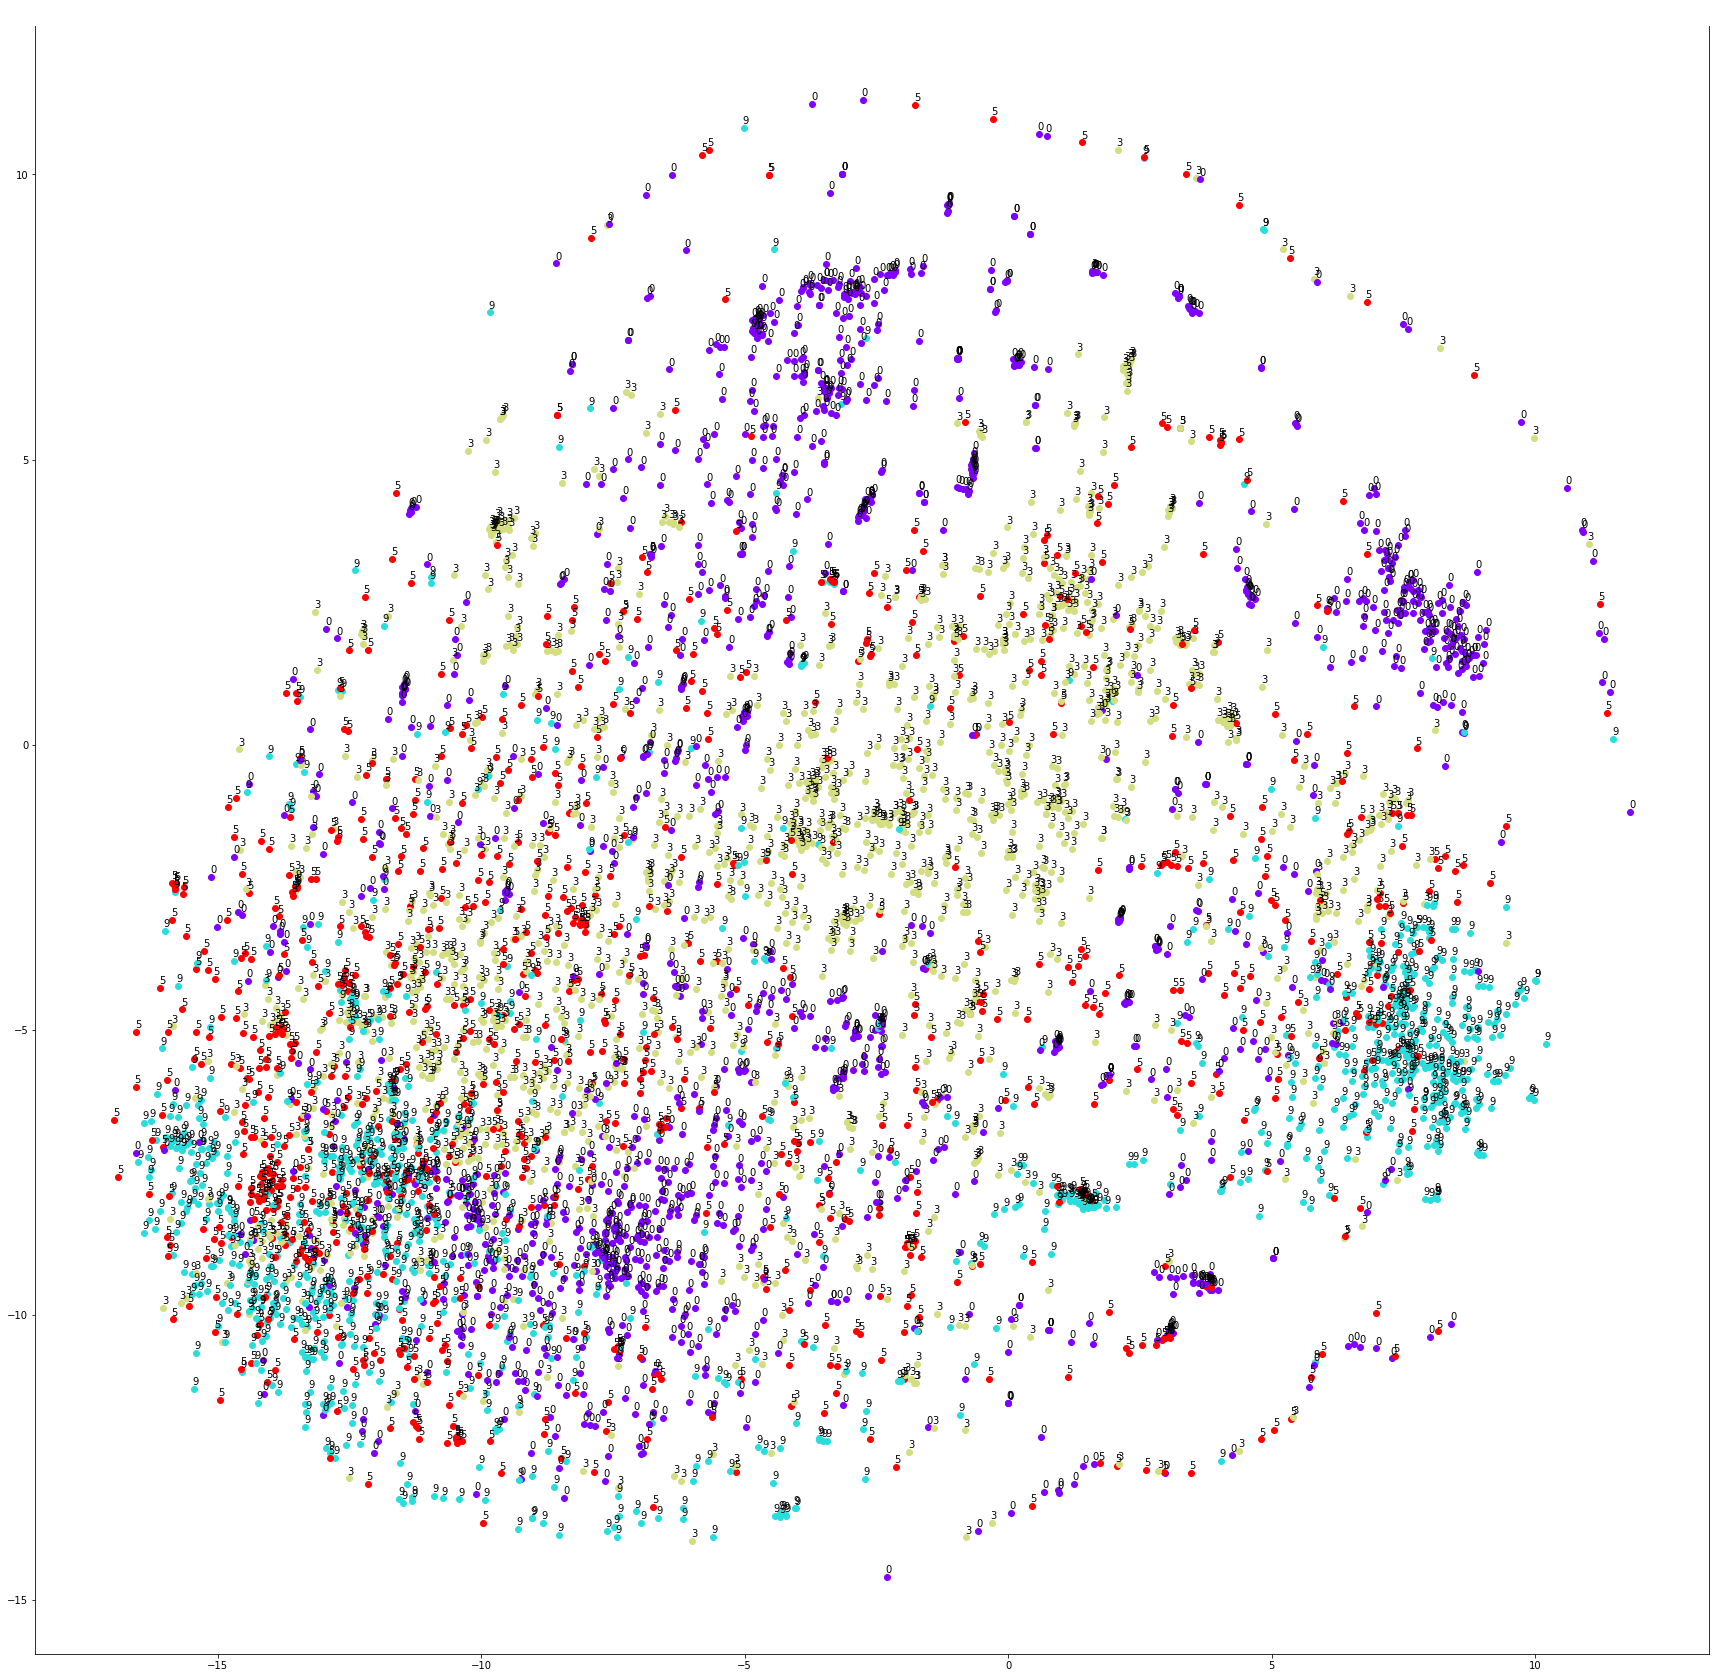
\includegraphics[width=0.49\linewidth]{figures/videos_1024_tsne_random_5000.png} &
  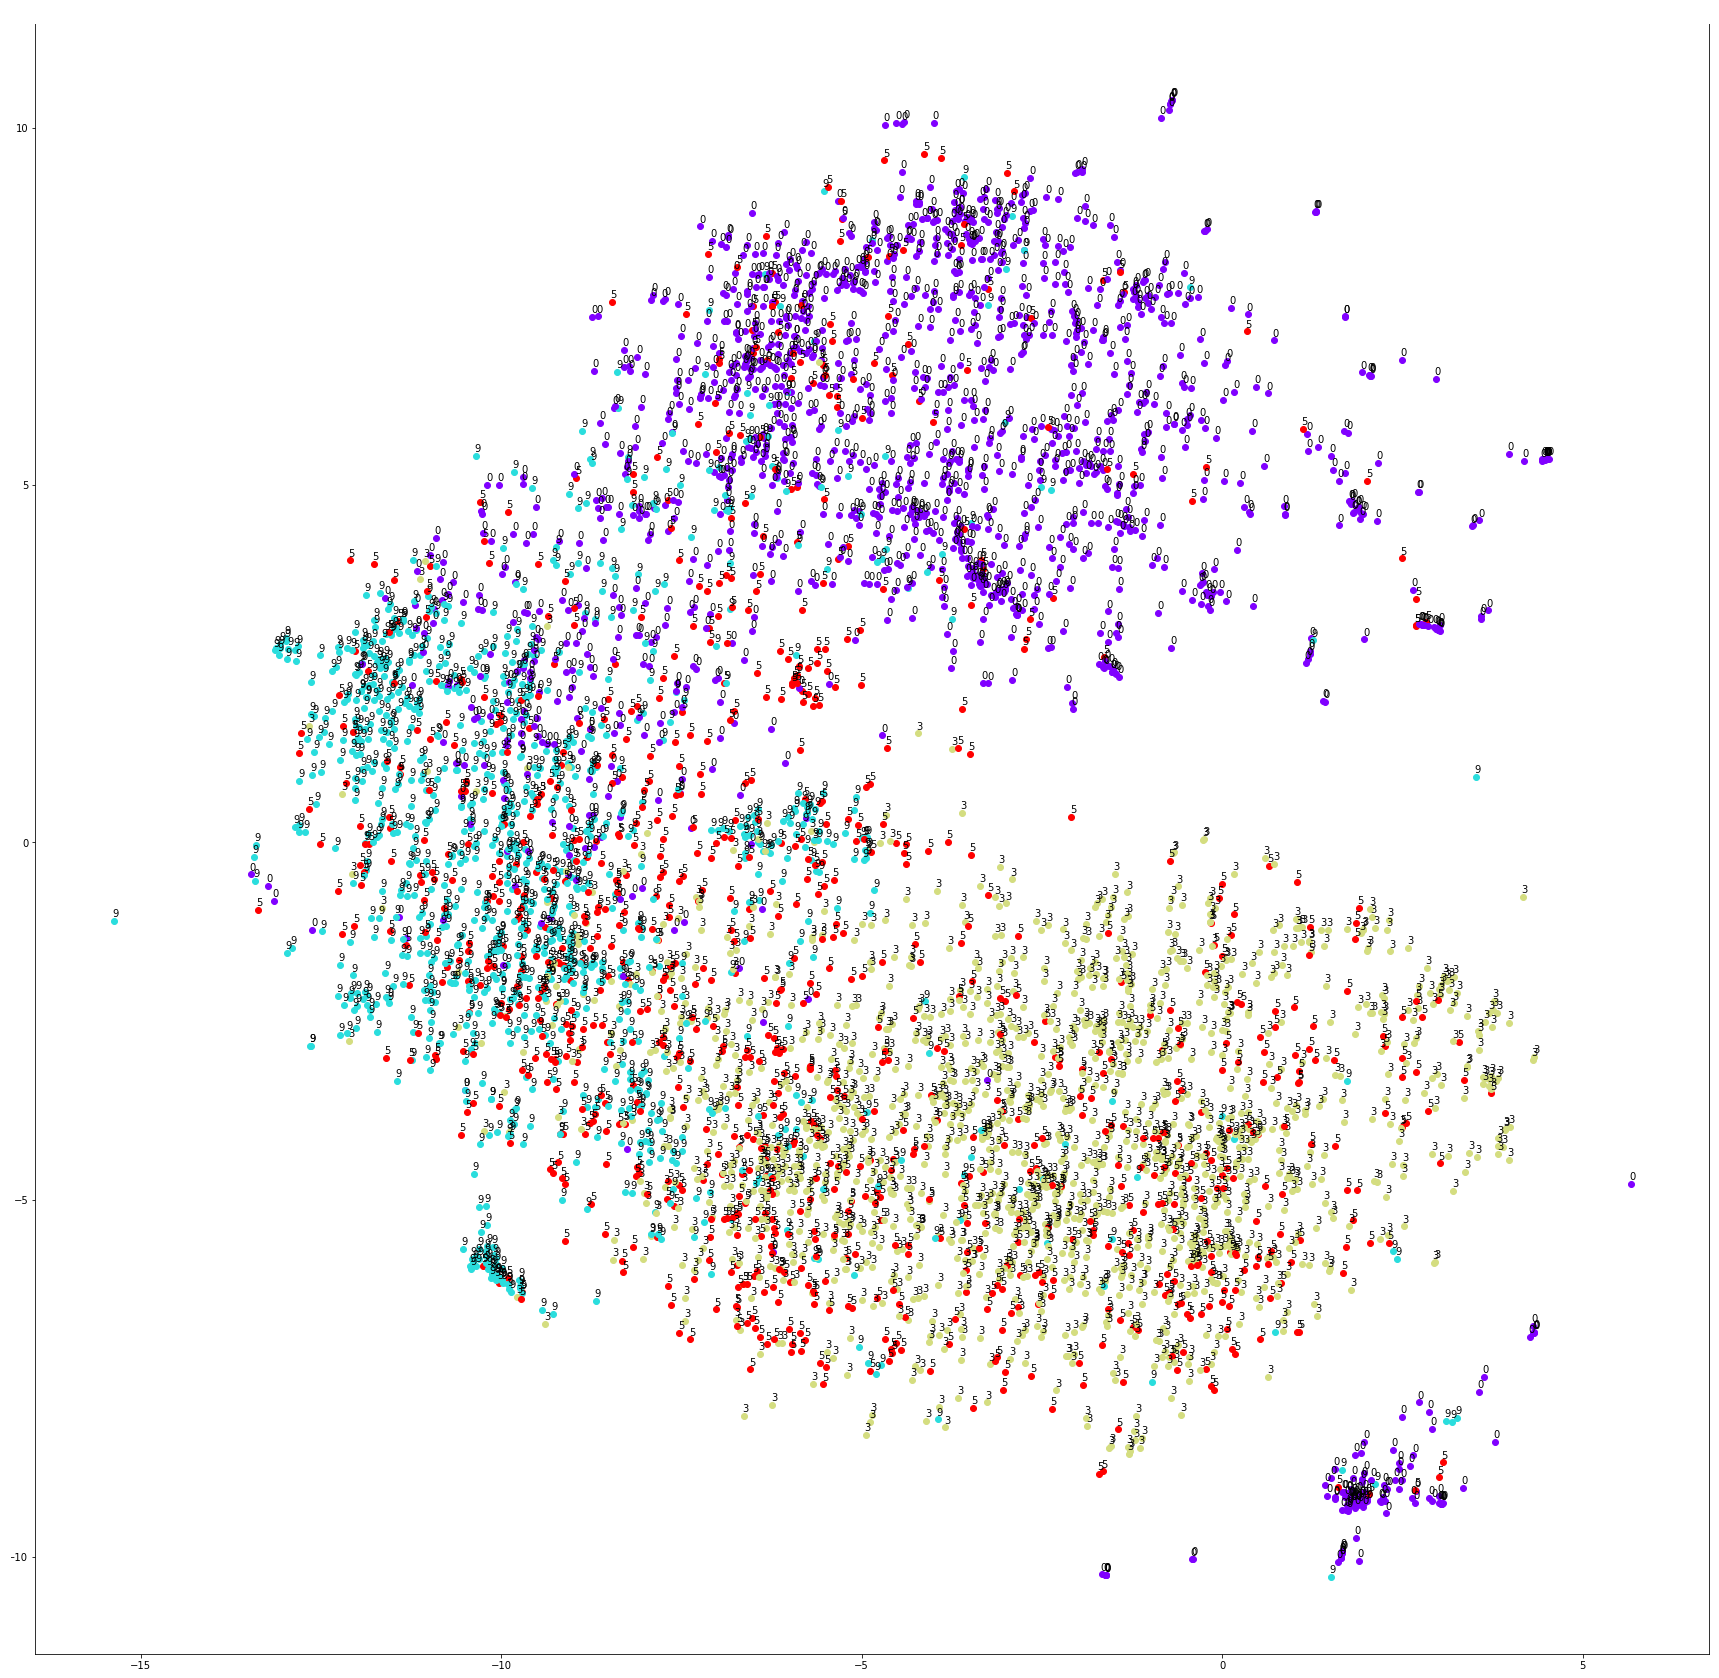
\includegraphics[width=0.49\linewidth]{figures/videos_128_tsne_random_5000.png} \\
   a) & b)\\
   \end{tabular}
   \begin{tabular}{cc}
  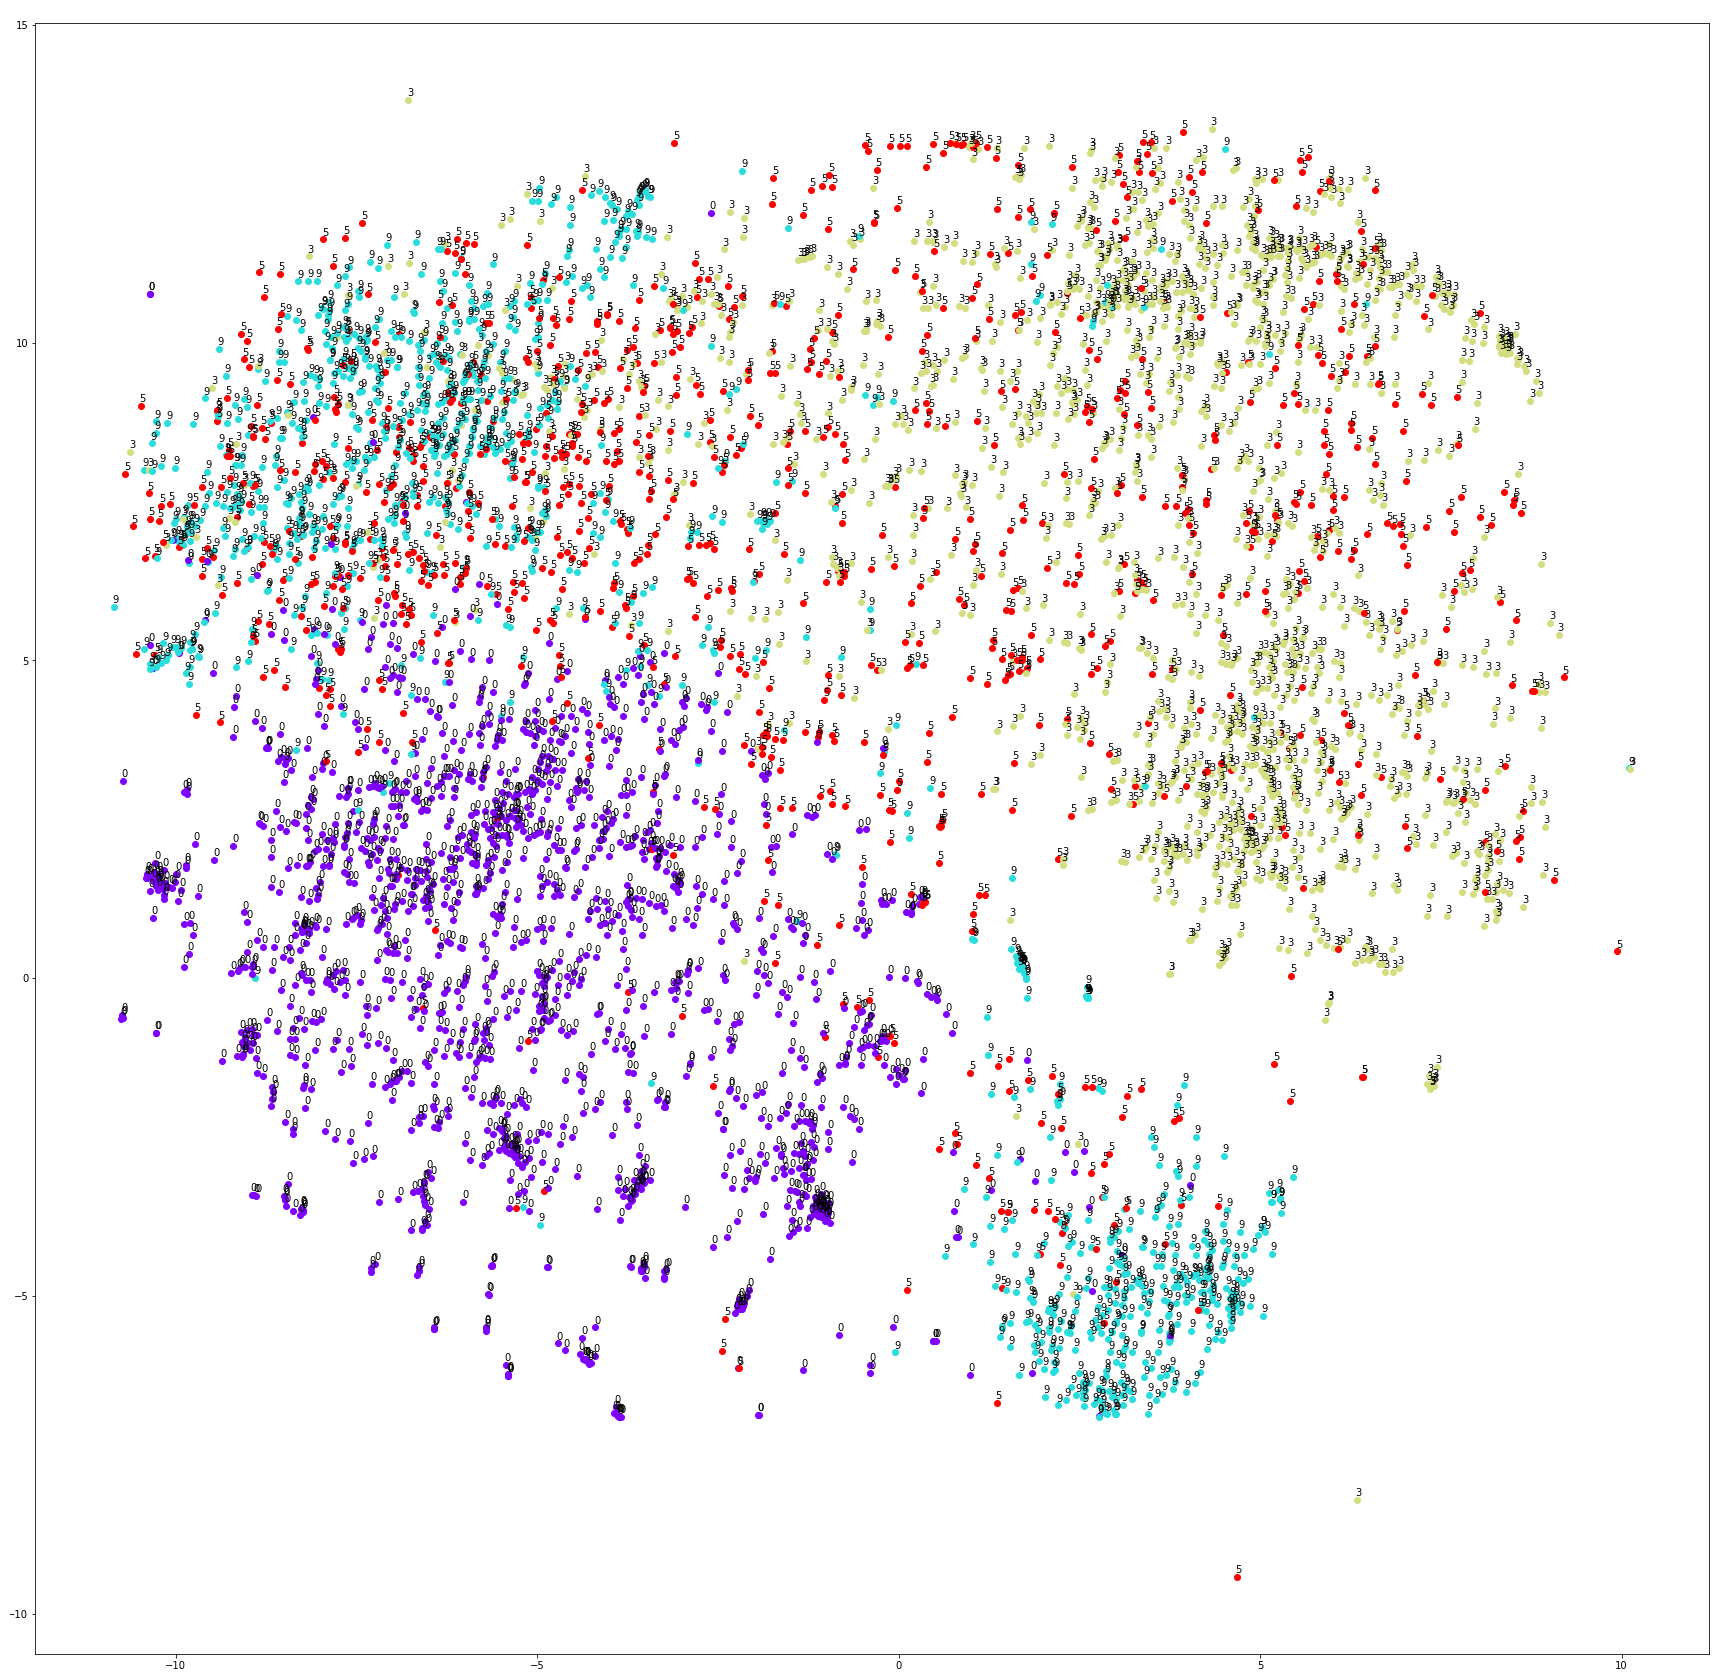
\includegraphics[width=0.49\linewidth]{figures/concat_128_tsne_random_5000.png} & 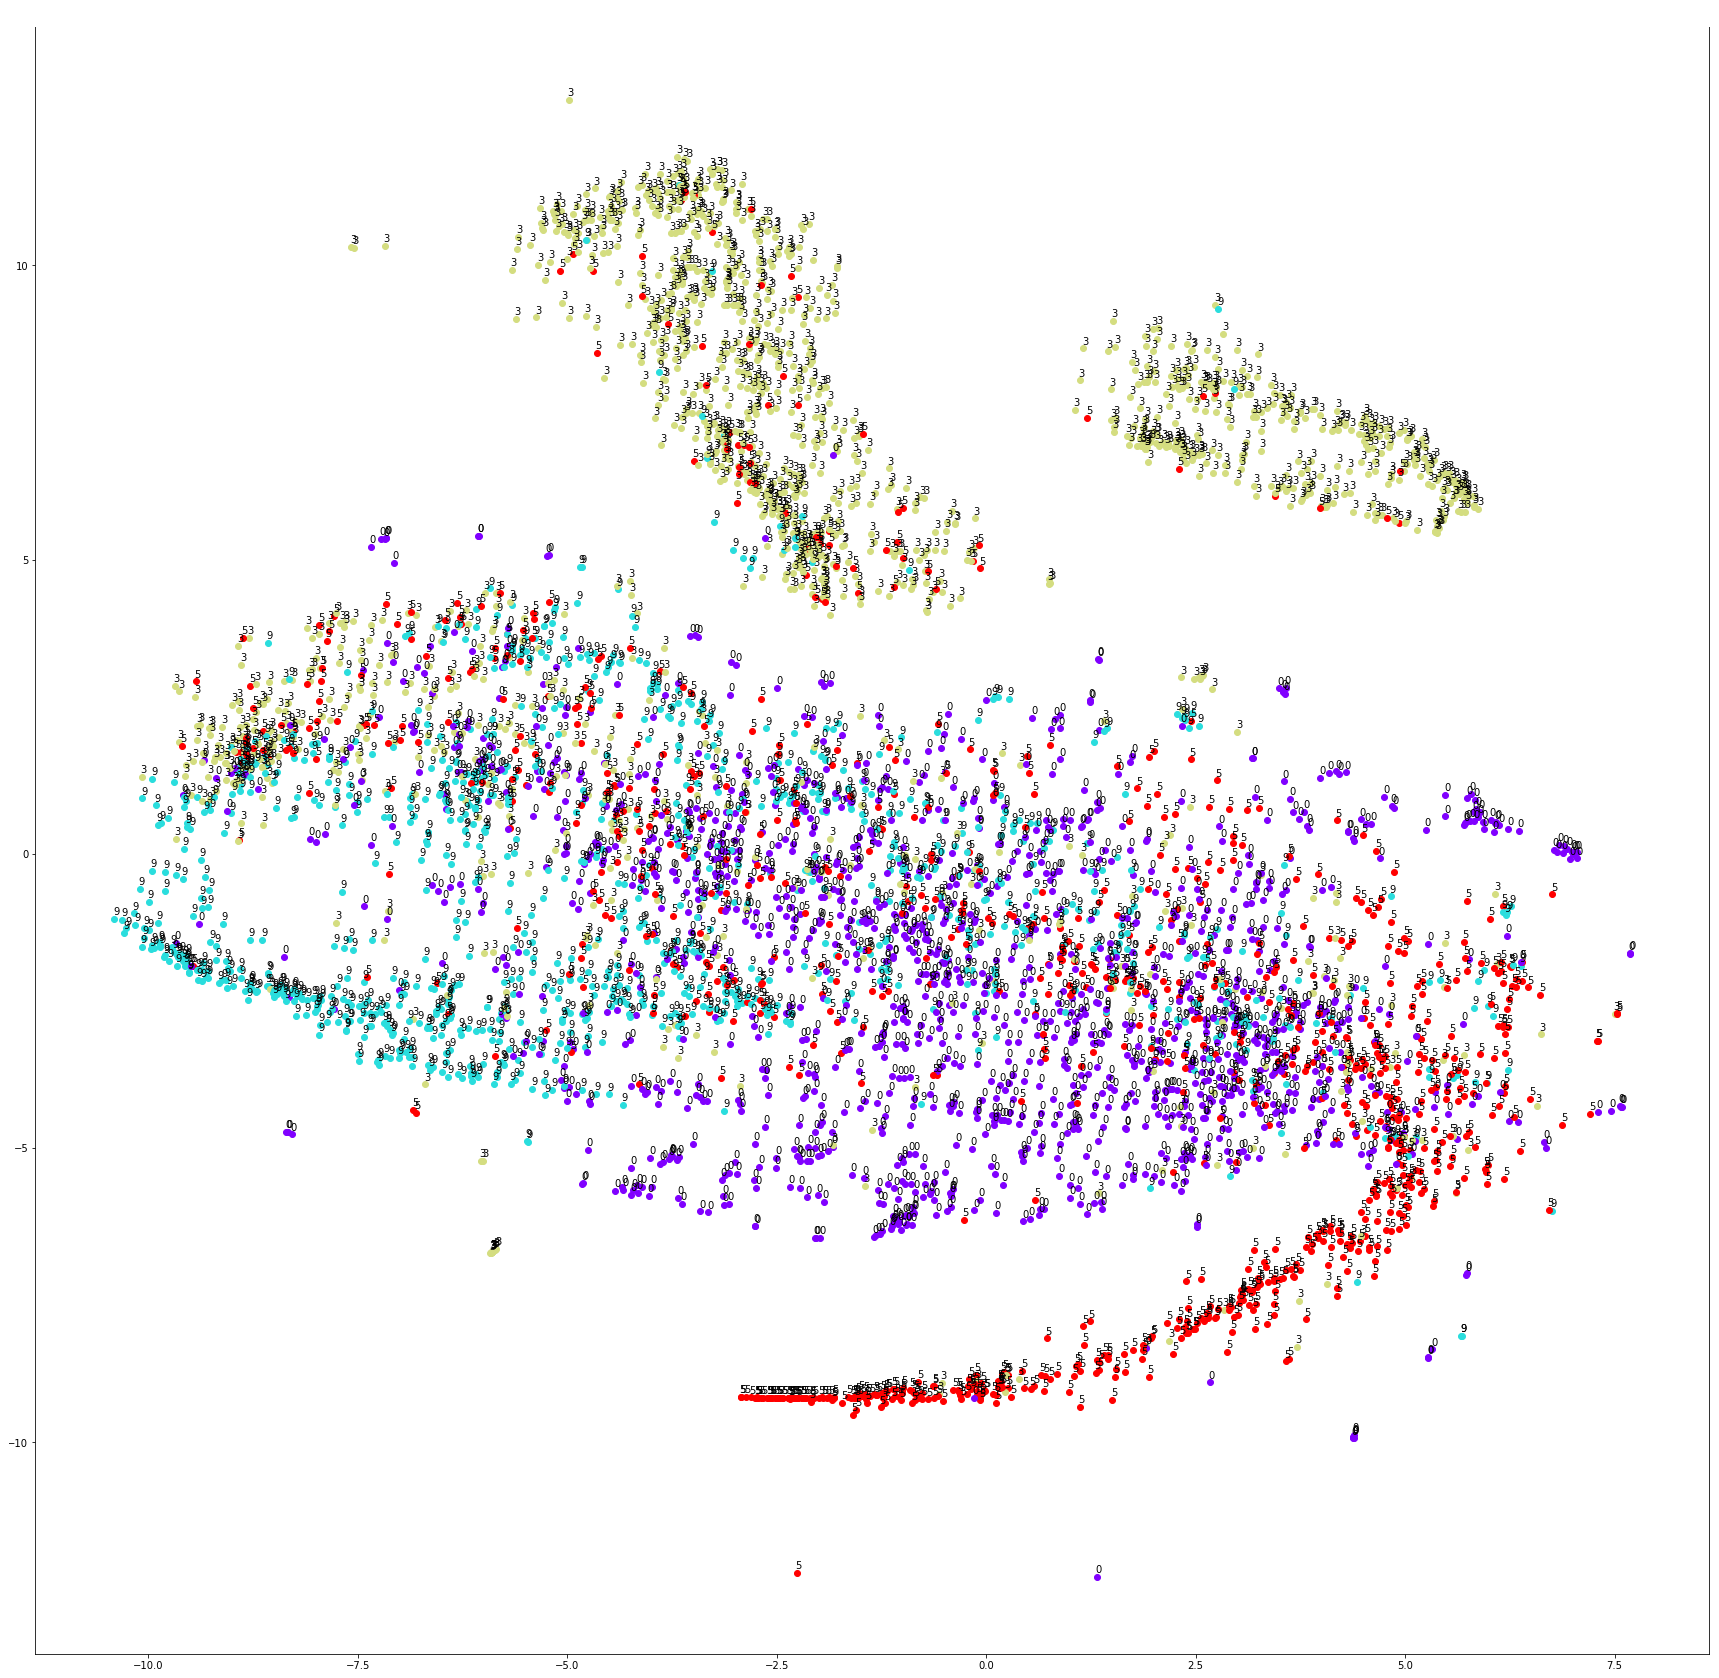
\includegraphics[width=0.49\linewidth]{figures/concat_alternating_128.png} \\
   c) & d)\\
   \end{tabular}
   \label{fig:kldplots}
  \captionof{figure}{t-SNE visualizations of 5000 randomly selected data points corresponding to Dance (Red), Concert (Yellow), Game (Purple) and Music (Blue). (a): Visualization for video features in their original dimensionality of 1024 dimensions. (b): Visualization of Video Features using \hyperref[variant1]{Variant improving video features using audio features}, (c): Visualization of Improved Concatenated Features fused to 128 dimensions using \hyperref[variant2]{Variant improving fused features using audio features} (d): Visualization of Improved Concatenated Features fused to 128 dimensions using \hyperref[variant3]{Variant using alternating classification error and KL divergence minimization}}
\end{center}




\begin{center}
\begin{figure}[h]
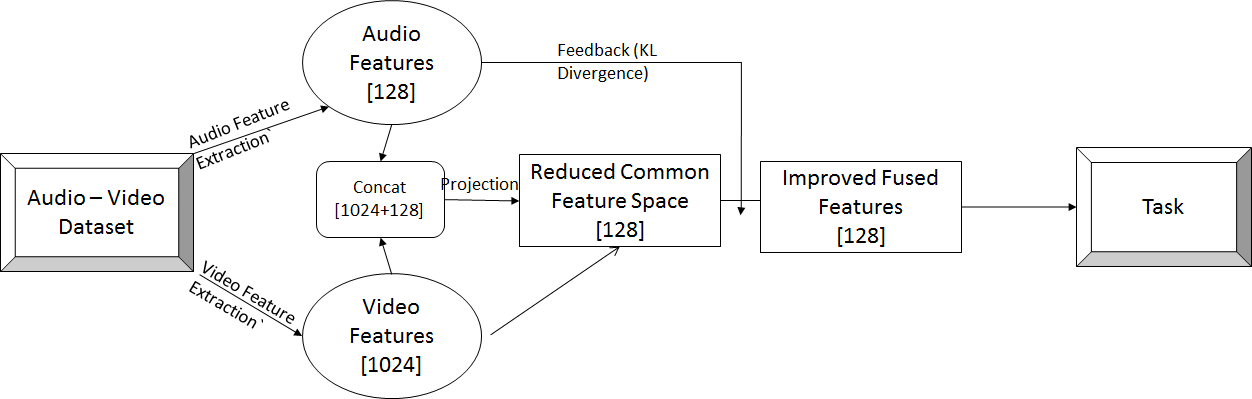
\includegraphics[width=1\textwidth]{figures/proposed.png}
\label{fig:genoverview}
\caption{General Overview of the Proposed Iterative K-L Divergence Minimization Algorithm}
\end{figure}
\end{center}

\section{Results}
Table [\ref{results-table}] tabulates the classification accuracy of different algorithms for the subset of the two datasets AudioSet \cite{audioset} \footnote{Subset of AudioSet  \cite{audioset}, that uses data points of only the top 4 most occurring labels}  and YouTube 8-M \cite{youtube8m} \footnote{Subset of YouTube 8-M \cite{youtube8m}, that uses data points of only the top 4 most occurring labels} . We created a subset of both the datasets by focusing only those data points that corresponds to labels among the top four most frequent classes. We used a 5 fold cross validation and kernalized SVM and extreme gradient boosting as classification algorithms, to test the performance of the transformed features as well as the original features. The improved classification performance of all the algorithms and specifically the proposed  iterative alternative classification  K-L divergence minimization as proposed in \ref{kl} does seem to strengthen our belief that a common representation of both the audio and video modalities is deemed to carry more information than each of them alone. 


\begin{table}[t]
  \caption{Classification accuracy for different algorithms for subset of AudioSet and YouTube 8M datasets}
  \label{results-table}
  \centering
  \begin{tabular}{lll}
    \toprule
    Features/ Dataset & AudioSet* & YouTube 8-M*\\
    \midrule
    Audio Features Only & 69.23\%  &  80.89\%     \\
    Video Features Only    & 69.23\% & 82.34\%      \\
    CCA (concatenation)     &  46.57\% & 81.54\%   \\
    CCA (sum)     &  42.31\% & 80.88\%   \\
    DCA     &68.1\% & 80.23\%   \\
    Audio Feedback on Video Features  &  TBC & 81.6\%   \\
    Audio + Video (concatenation) with Audio Feedback   & TBC & \textbf{83.91}\%   \\
    \bottomrule
  \end{tabular}
\end{table}

\section{Conclusion}
The proposed alternating iterative method succeeds in learning a common projection feature space at least for the audio and video features from a video. It shows that the modality that has a stronger confidence, can be used to strengthen the learned fused feature space representations. Though we have tried for reduced subset of the labels, the proposed technique should generalize well for the entire dataset. As a next future step, it would be interesting to see the effect of Kernel methods during the feedback mechanism of our algorithm. It would also be interesting to see for different probability measures which may further improve the performance.   
% \section{Final instructions}

% Do not change any aspects of the formatting parameters in the style
% files.  In particular, do not modify the width or length of the
% rectangle the text should fit into, and do not change font sizes
% (except perhaps in the \textbf{References} section; see below). Please
% note that pages should be numbered.

% \section{Preparing PDF files}

% Please prepare submission files with paper size ``US Letter,'' and
% not, for example, ``A4.''

% Fonts were the main cause of problems in the past years. Your PDF file
% must only contain Type 1 or Embedded TrueType fonts. Here are a few
% instructions to achieve this.

% \begin{itemize}

% \item You should directly generate PDF files using \verb+pdflatex+.

% \item You can check which fonts a PDF files uses.  In Acrobat Reader,
%   select the menu Files$>$Document Properties$>$Fonts and select Show
%   All Fonts. You can also use the program \verb+pdffonts+ which comes
%   with \verb+xpdf+ and is available out-of-the-box on most Linux
%   machines.

% \item The IEEE has recommendations for generating PDF files whose
%   fonts are also acceptable for NIPS. Please see
%   \url{http://www.emfield.org/icuwb2010/downloads/IEEE-PDF-SpecV32.pdf}

% \item \verb+xfig+ "patterned" shapes are implemented with bitmap
%   fonts.  Use "solid" shapes instead.

% \item The \verb+\bbold+ package almost always uses bitmap fonts.  You
%   should use the equivalent AMS Fonts:
% \begin{verbatim}
%    \usepackage{amsfonts}
% \end{verbatim}
% followed by, e.g., \verb+\mathbb{R}+, \verb+\mathbb{N}+, or
% \verb+\mathbb{C}+ for $\mathbb{R}$, $\mathbb{N}$ or $\mathbb{C}$.  You
% can also use the following workaround for reals, natural and complex:
% \begin{verbatim}
%    \newcommand{\RR}{I\!\!R} %real numbers
%    \newcommand{\Nat}{I\!\!N} %natural numbers
%    \newcommand{\CC}{I\!\!\!\!C} %complex numbers
% \end{verbatim}
% Note that \verb+amsfonts+ is automatically loaded by the
% \verb+amssymb+ package.

% \end{itemize}

% If your file contains type 3 fonts or non embedded TrueType fonts, we
% will ask you to fix it.


% \subsection{Margins in \LaTeX{}}

% Most of the margin problems come from figures positioned by hand using
% \verb+\special+ or other commands. We suggest using the command
% \verb+\includegraphics+ from the \verb+graphicx+ package. Always
% specify the figure width as a multiple of the line width as in the
% example below:
% \begin{verbatim}
%    \usepackage[pdftex]{graphicx} ...
%    \includegraphics[width=0.8\linewidth]{myfile.pdf}
% \end{verbatim}


% See Section 4.4 in the graphics bundle documentation
% (\url{http://mirrors.ctan.org/macros/latex/required/graphics/grfguide.pdf})

% A number of width problems arise when \LaTeX{} cannot properly
% hyphenate a line. Please give LaTeX hyphenation hints using the
% \verb+\-+ command when necessary.

\subsubsection*{Acknowledgments}
We would like to thank Prof. Lior Horesh and Prof. Julie E. Novak for their encouragement, guidance, and teaching. We would also like to thank Google Inc. for the amazing and well designed datasets. Without their support, this project would not have been possible.


\bibliography{references}
\bibliographystyle{abbrv}

\end{document}
